\section{导引}
深度学习模型现在可以识别图像、处理自然语言和在策略游戏中击败人类。
现在,将智能应用程序部署到广泛的设备上,比如从云服务器到自动驾驶汽车和嵌入式设备的需求越来越大。
因为硬件的多样性,包括嵌入式CPU、GPU、FPGA和ASIC(例如TPU),将深度学习工作负载映射到这些设备的工作是复杂的。
这些硬件在内存组织、计算功能单元等方面上是不同的,如图\ref{fig:mem subsys arch}所示。

\begin{figure}[htbp]
    \centering
    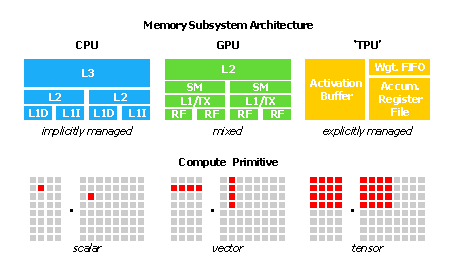
\includegraphics[width=.9\linewidth]{tvm/mem_subsys_arch}
    \caption{\label{fig:mem subsys arch}CPU、GPU、和类TPU加速器需要不同的片上内存架构和计算原语。
    这样的差异可以通过生成优化代码来被解决。}
\end{figure}

当前的深度学习框架,如TensorFlow、MXNet、Caffe和PyTorch,依赖于计算图中间表示来实现优化,例如,自动微分和动态内存管理。
然而,图级别优化通常太高层,无法处理特定硬件后端的算子级别转换。这些框架大多专注于服务端GPU,
并将特定目标优化委托给高度工程化的供应商提供的库。这些算子库需要大量的手动优化,因此过于专业化而且生态封闭,
以至于不容易移植到其他硬件上。为不同的硬件后端提供不同的深度学习框架支持目前需要大量的工程工作。即使对于支持的后端,
框架也必须做出艰难的选择:
\begin{enumerate*}
    \item 避免使用生成新算子的图级别优化,
    \item 使用这些新算子的未优化实现。
\end{enumerate*}

为了对于不同的硬件后端同时启用图级别和算子级别优化,我们采用一种完全不同的端到端方法。
我们构建了TVM,这是一个编译器,它从现有的框架中获取一个高层次的深度学习程序,并为不同的硬件后端生成优化过的底层代码。
为了吸引用户,TVM需要在不同的硬件后端提供与众多手动优化的算子库相竞争的性能。这一目标要求解决下述的关键挑战:

\paragraph{利用特定的硬件特性和抽象}
深度学习加速器引入了优化的张量计算原语,而GPU和CPU则不断改进其处理单元。这在为给定的算子生成优化代码
带来了重大挑战。硬件指令的输入是多维的,具有固定或可变的长度;它们使用不同的数据布局;它们对内存层次结构有特殊的要求。
该系统必须有效地利用这些硬件原语来获得加速。此外,加速器设计通常更希望精简控制,并将复杂的调度移到到编译器中。
对于专用加速器,系统现在需要生成显式控制流水线依赖来隐藏内存访问延迟的代码,这是硬件为CPU和GPU执行的工作。

\paragraph{利用大搜索空间来优化}
另一个挑战是在不手动调整算子的情况下生成高效的代码。内存访问、线程特性和新硬件原语的组合为生成的代码
(例如循环分块和排序、缓存、循环展开)创建了巨大的配置空间,如果我们实现黑盒自动优化,这将产生巨大的搜索成本。
一种方法是采用预先定义的代价模型来指导搜索,但由于现代硬件的复杂性日益增加,建立一个准确的代价模型是困难的。
此外,这样的方法将要求我们为每种硬件类型构建单独的代价模型。

TVM通过三个关键模块来应对这些挑战。
\begin{enumerate*}
    \item 我们引入一种张量表达式语言来构建算子,并提供程序转换原语,这些原语通过各种优化生成不同版本的程序。
    该层扩展了Halide的计算/调度(Schedule)分离概念,将目标硬件内部细节与转换原语分离,从而支持新的加速器。
    此外,我们引入了新的转换原语以解决与GPU相关的挑战,并支持部署到专用加速器。
    然后我们可以为给定的算子,应用不同的程序转换序列来形成一个丰富的合法程序集合。
    \item 我们引入了一个自动化的程序优化框架来搜索优化的张量算子。该优化器依赖于一个基于机器学习的的代价模型,
    随着我们对一个硬件收集的数据越来越多,该具有自适应能力的代价模型将自我进步。
    \item 在自动代码生成器的基础上,我们引入了一个图重写器,它充分利用了图级别和算子级别的优化。
\end{enumerate*} 

通过结合这三个模块,TVM可以从现有的深度学习框架中获取模型,联合执行高级和低级优化,并为专用硬件后端生成的优化的代码,
例如CPU、GPU和基于FPGA的专用加速器。

这篇文章主要做出了如下的贡献:

\begin{itemize}
    \item 我们确定了在跨不同硬件后端为深度学习工作负载提供性能可移植性方面的主要优化挑战。
    \item 我们引入了新的调度原语,它利用了跨线程内存重用、新硬件细节和延迟隐藏的优势。
    \item 我们提出并实现了一个基于机器学习的优化系统,以自动探索和搜索优化的张量算子。
    \item 我们构建了一个端到端的编译和优化栈,允许将特定高级框架(包括TensorFlow、MXNet、PyTorch、Keras、CNTK)
    的深度学习工作负载部署到不同的硬件后端(包括CPU、服务端GPU、移动端GPU和基于FPGA的加速器)。
    开源的TVM现在在几家大公司内部投入生产使用。
\end{itemize}

我们在一个服务端GPU、一个嵌入式GPU、一个嵌入式CPU和一个FPGA加速器上用真实的工作负载来评估TVM。
实验结果表明,TVM在多后端提供了可移植的性能,相比现有的手工优化的框架获得了1.2到3.8的加速比。
